\chapter{Fantastic Errors and Where to Find Them (Debugging)}

\section{Introduction}

In the previous lab sessions you wrote some code. Most probably, your code didn't work at first. What you had is called a bug, and it is the nemesis of programmers since times untold. The term has been used in as early as $1878$\footnote{https://en.wikipedia.org/wiki/Debugging}. Back in the days computers were room-sized heavy machines, some bugs were literally bugs stuck in the machinery. Nowadays, bugs mostly live in our code.

\begin{marginfigure}
\centering
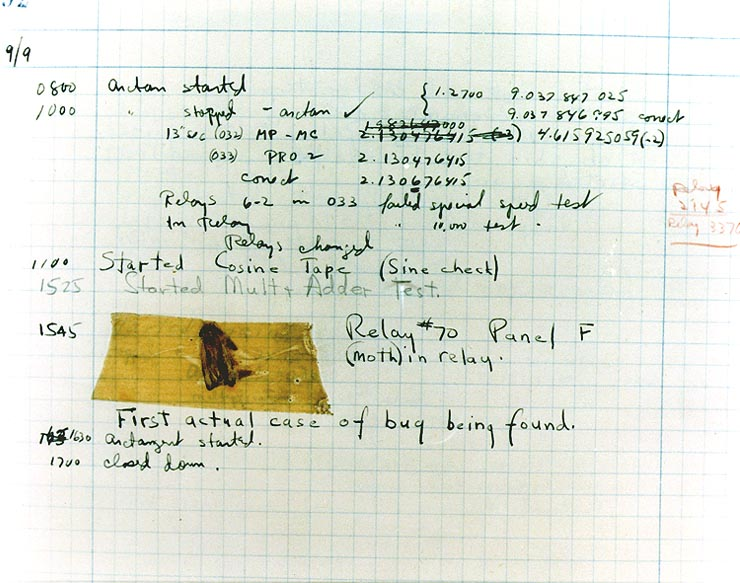
\includegraphics[width=.9\linewidth]{images/bug.jpg}
\caption{An early documented bug, found in the Mark II computer, 1947. Courtesy of the Naval Surface Warfare Center, Dahlgren, VA., 1988. / Public domain}
\end{marginfigure}

In this lesson we'll learn about bugs and how to fight them. 

\begin{definition}
\emph{debugging} is the process of identifying and removing errors from computer hardware or software.
\end{definition}

Debugging is like detective work, and it is a skill that can be trained, just like writing code. But before we start debugging, we first need to learn the basic terminology, and the way DrJava will report bugs and other problems to us. Let's start with a classification of problems in a program:

\begin{definition}
\leavevmode\newline
\begin{itemize}
    \item a \emph{compilation error} is an problem encountered during the compilation process, before running the code. A code with compilation errors cannot be run.
    \item a \emph{runtime error} is encountered while the code is running, after it has been successfuly compiled. It typically represents a serious problem that should stop the code once encountered.
    \item an \emph{exception} is also encountered while the code is running. It typically represents a problem that an application can try to recover from and keep running.
    \item a \emph{bug} is a flaw in a program that causes it to behave in unintended ways. This can include the program encountering errors or exceptions, but can also lead to a program that runs without either of these errors but in an incorrect way, in which case we will call it a \emph{silent bug}.
\end{itemize}
\end{definition}

The exact distinction between errors and exceptions is soft, and varies between languages. The Java language also distinguishes between two types of exceptions, checked and unchecked, but we won't go over the distinction here.

\section{Compilation Errors}

Let's look at the following example:

\begin{example}
What's wrong with the following code?

\begin{code}
public class Snippet{
    public static void main(String []args){
        int x = 5.5;
    }
}
\end{code}
\end{example}

This code will result in a compilation error. Let's look at the message DrJava will display when trying to compile this code, in figure~\ref{fig:type_mismatch}.

\begin{figure}[h!]
\centering
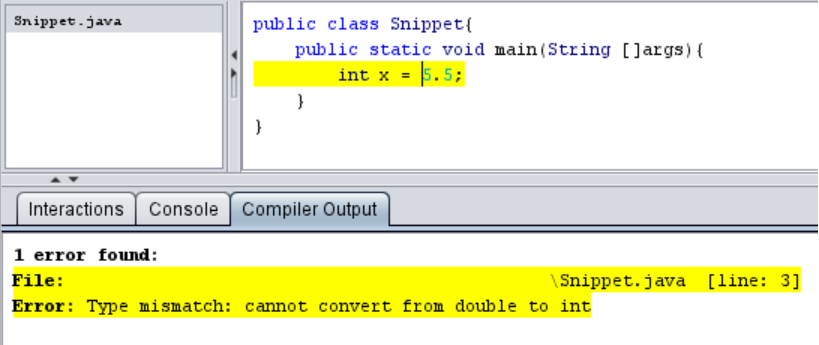
\includegraphics[scale=0.8]{images/incompatible_types.PNG}
\caption{An incompatible type error.}
\label{fig:type_mismatch}
\end{figure}

The line the compiler got stuck at is highlighted in yellow, helping us focus on the likely cause of the error. In the "Compiler Output" window, we see three lines that give us information on our problem:

\begin{enumerate}
    \item "1 error found:"
    Sometimes the compiler is able to put aside an error and keep trying to compile the rest of the code, so we could see as much errors we made as possible. The number of errors the compiler was manage to find is listed here, in our case just one.
    \item "File: ...\\Snippet.java [line: 3]" 
    The first part of the line is the path of the file where the error was found (some part omitted). If our code spanned multiple files, this would help us find the right one to focus on.
    The second part of the line tells us the line number where the error was found. If our code is long this would help us scroll to the relevant part.
    \item "Error: Type mismatch: cannot convert from double to int".
    This part tells us what kind of error was found on this line. In this case, it tells us that the error was a "type mismatch" -- this means that we were trying to assign some value to a variable of another value, in a way that does not make sense. The rest of the line explains why this assignment did not make sense -- we were assigning a double value, $5.5$, to an $int$ variable, but a double value can't be converted to an $int$ in a safe manner.
\end{enumerate}

By focusing our attention on the location of the error, and telling us what kind of error it was, the compiler helps us identify and fix it quickly. Sometimes, however, errors are trickier to find, as in this example:

\begin{example}
What's wrong with the following code?

\begin{code}
public class Snippet{
    public static void main(String []args){
        int x = 5.5;
    
}
\end{code}
\end{example}

This code has the same error as the previous one, but there's another problem with it - the $\}$ sign that was supposed to end the $main$ block is missing. Let's look at the compiler output for this code, in figure~\ref{fig:syntax_error}:

\begin{figure}[h!]
\centering
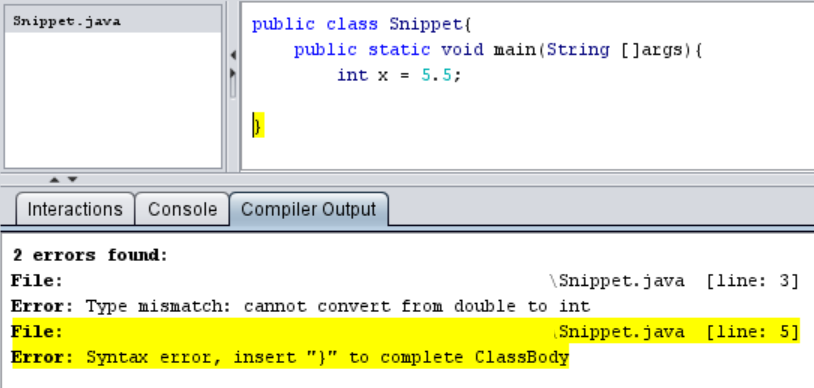
\includegraphics[scale=0.8]{images/syntax_error.PNG}
\caption{A new syntax error joins the previous error.}
\label{fig:syntax_error}
\end{figure}

First, notice that the compiler was able to found both errors. If we click on the two lines corresponding to each error, DrJava will highlight the relevant row in our code. 

The new error we encountered is called a syntax error. Like any spoken and programming language, Java has a syntax that's required to build meaningful commands. This includes ending statements with a semicolon $;$, closing any open $"$, $\{$, $($ and $[$ and more (we'll see more examples in the assignment). In our case, the block of the $main$ method has to start with a $\{$ and end with a $\}$. If not, the compiler won't be able to figure out where the $main$ method ends.

This is exactly what is happening here -- the compiler can't know what the $\}$ is closing here, it just finished scanning the entire code and realized it is still missing one $\}$. In more complicated code, the compiler might not be able to point us close enough to the problematic line, so with syntax errors we need to be extra careful going over our code.

\section{Runtime Errors and Exceptions}

Problems that happen during a program's run are generally more difficult than compilation problems. That is because often these problems \emph{might} happen, but don't \emph{necessarily} happen. Moreover, a program might reach a certain line of code multiple times during its execution. This makes it harder to figure out when our program failed, and so why it failed.

Let's take a look at several examples of runtime errors and exceptions, and the information that Java (through DrJava) gives us to help investigate them.

\begin{example}
Look at the following program's code. Does it do what it claims to do? Can it run into a problem?

\begin{code}
import java.util.Scanner;

public class Snippet{
    public static void main(String []args){
      // Takes a number as input from the user, and prints the number back with a message.
      Scanner input = new Scanner(System.in);
      String token = input.next();
      int num = Integer.parseInt(token);
      System.out.println("The number you chose is: " + num);
    }
}
\end{code}
\end{example}

This code compiles without a problem, and seems to do what it claims -- it scans an input from the user, treats it as a number, and prints it back with a message. Now, let's look at two possible executions of the program, shown in figure~\ref{fig:number_format_error}

\begin{figure}[h!]
\centering
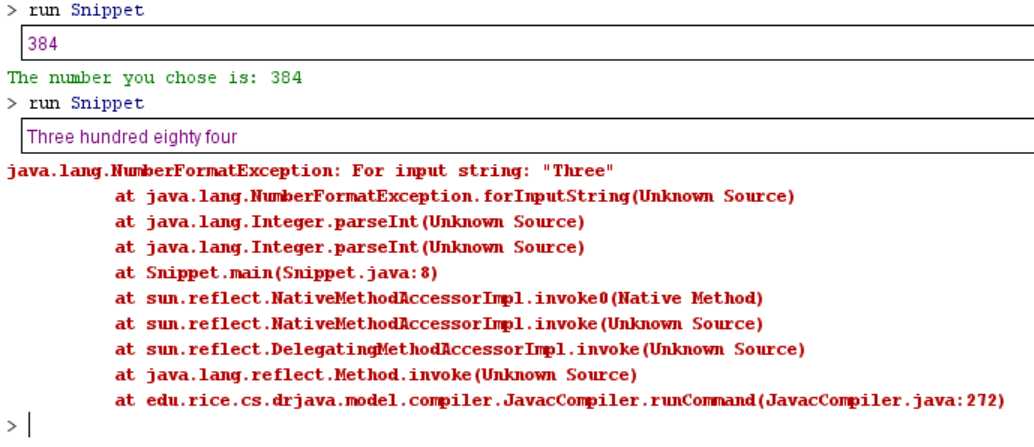
\includegraphics[scale=0.7]{images/number_format_exception.PNG}
\caption{Two executions of the program, one causing an exception.}
\label{fig:number_format_error}
\end{figure}

The first time the program was run, the user wrote $384$ as an input, and the program ran fine. The second time, however, the user wrote the number using words. Integer.parseInt wasn't able to parse the token it got, "Three", and \emph{threw} an exception. Our program didn't recover from the exception, and instead terminated.

The first red line below our execution prompt lists the type of exception and its details. The exception was NumberFormatException (ignore the prefix "java.lang."). The rest of the line details that the problem was encountered given the input "Three".

The red lines that follow are called the \emph{stack trace}, and they are very important for understanding when and where our code failed. Before we read them, let's do a little imagination exercise. Think of running of a program as a little turtle traveling code lines and executing them (this is slightly inaccurate, but close enough!). Figure ~\ref{fig:turtles} shows the journey of the turtle throughout the code in the last example, before it crashes with the exception we saw. 

\begin{figure}[h!]
\begin{subfigure}{1\textwidth}
  \centering
  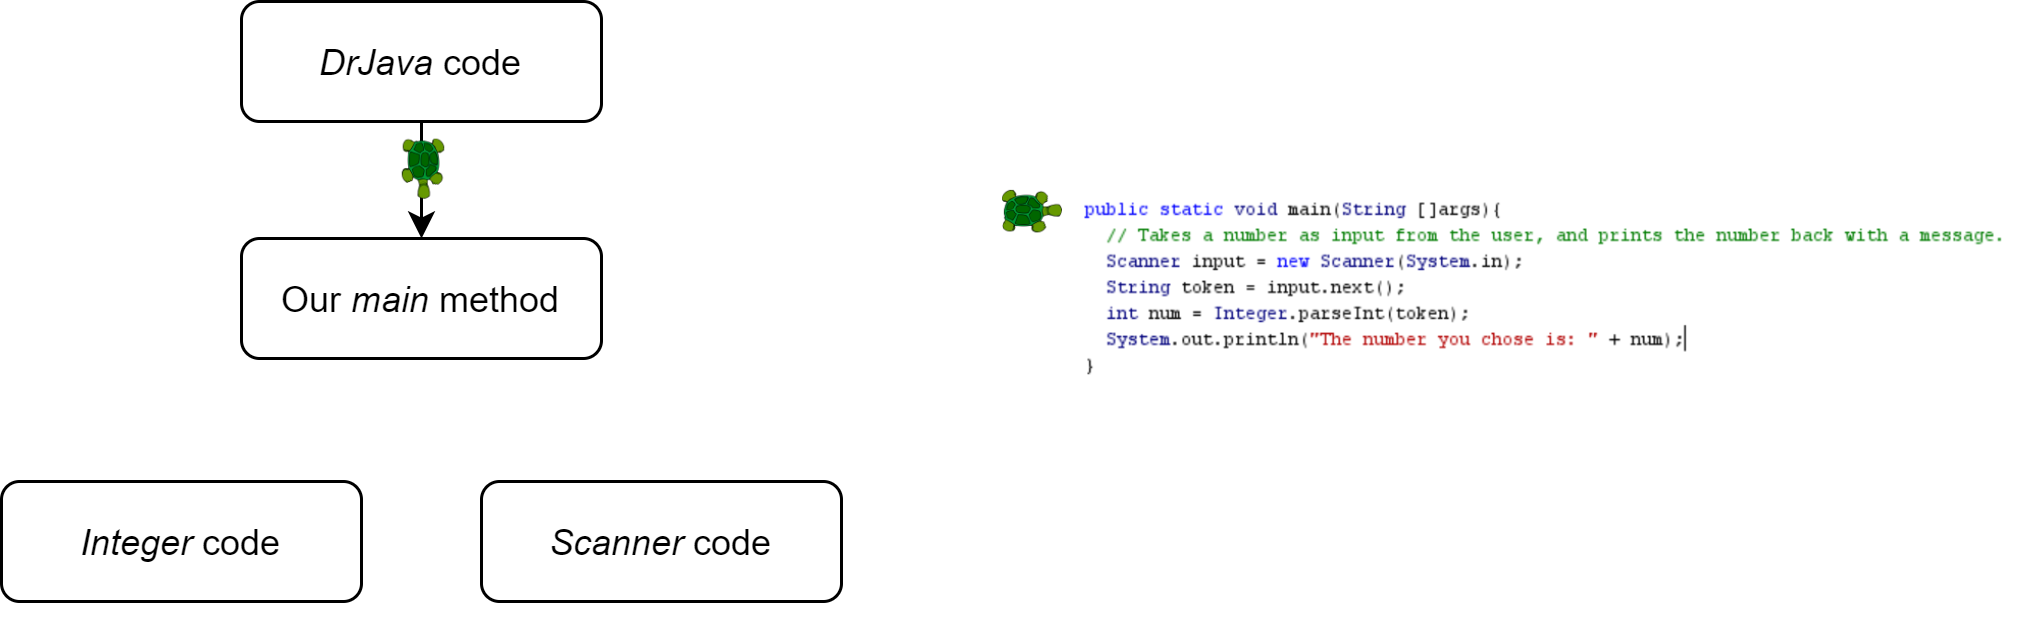
\includegraphics[width=1\textwidth]{images/code_turtle_1.png}
  \caption{}
  \label{fig:sturtle1}
\end{subfigure}%

\begin{subfigure}{1\textwidth}
  \centering
  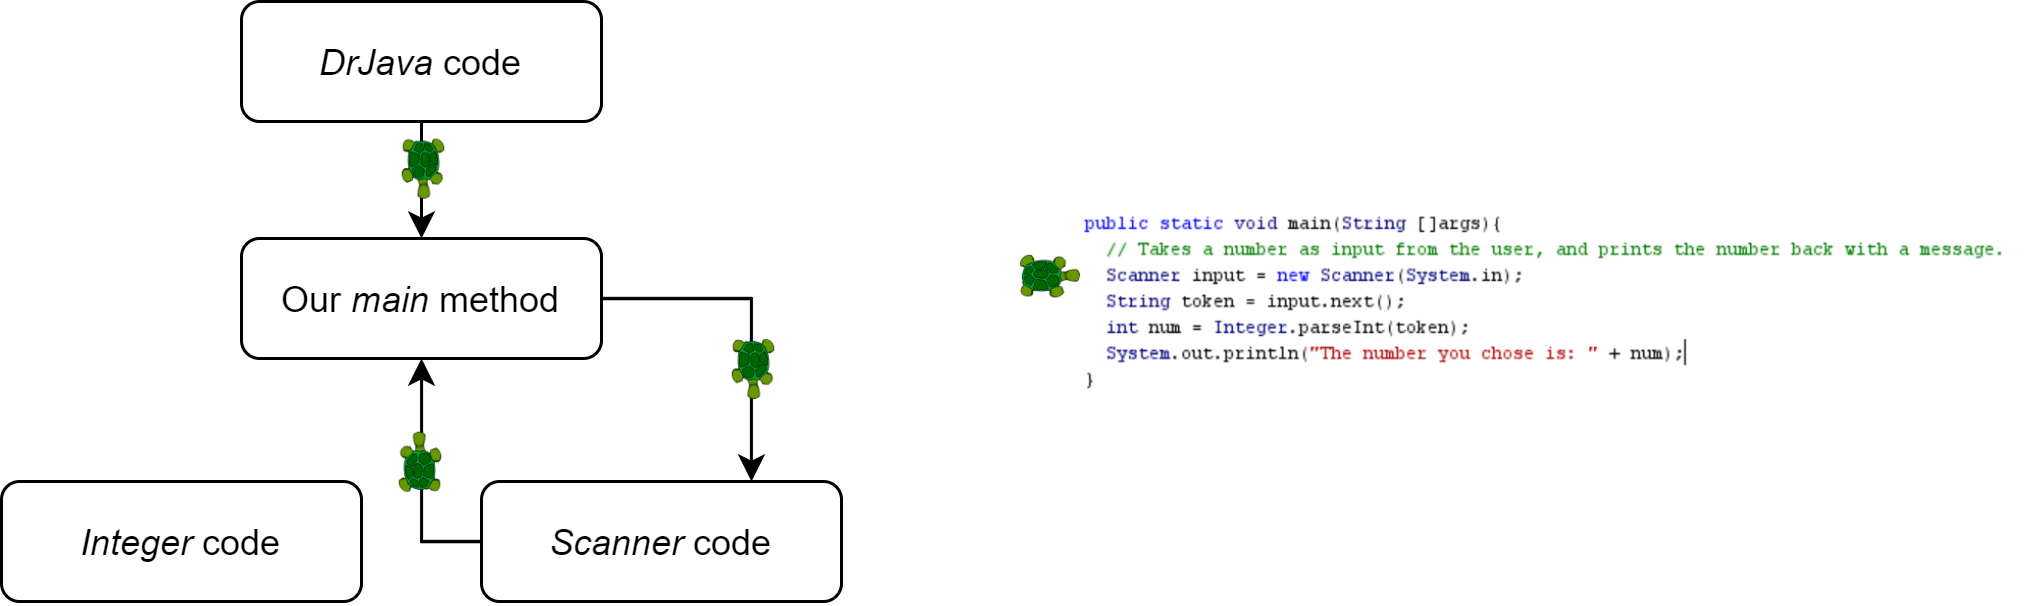
\includegraphics[width=1\textwidth]{images/code_turtle_2.png}
  \caption{}
  \label{fig:sturtle2}
\end{subfigure}%

\begin{subfigure}{1.\textwidth}
  \centering
  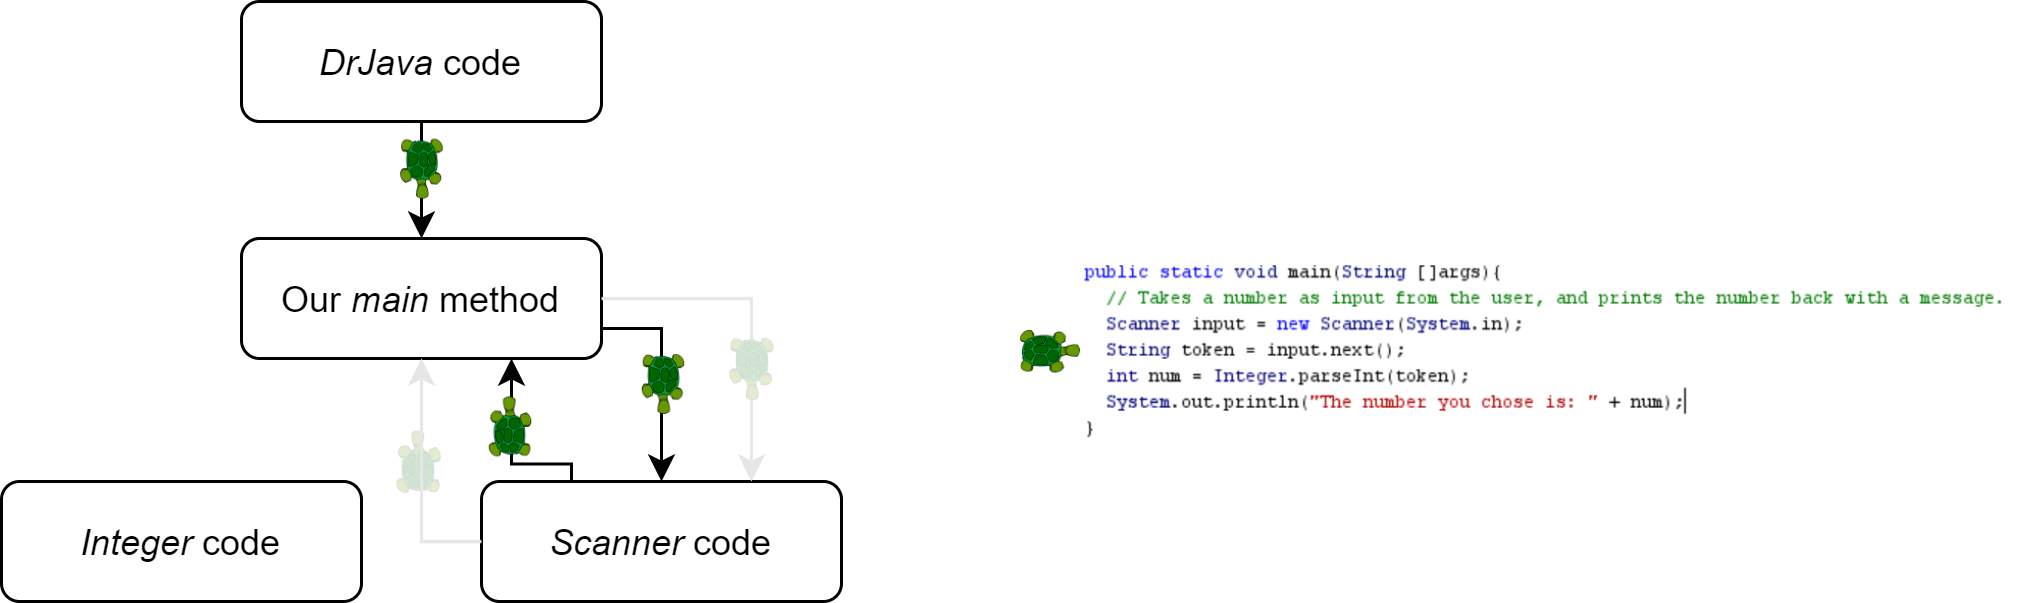
\includegraphics[width=1\textwidth]{images/code_turtle_3.png}
  \caption{}
  \label{fig:sturtle3}
\end{subfigure}%

\begin{subfigure}{1.\textwidth}
  \centering
  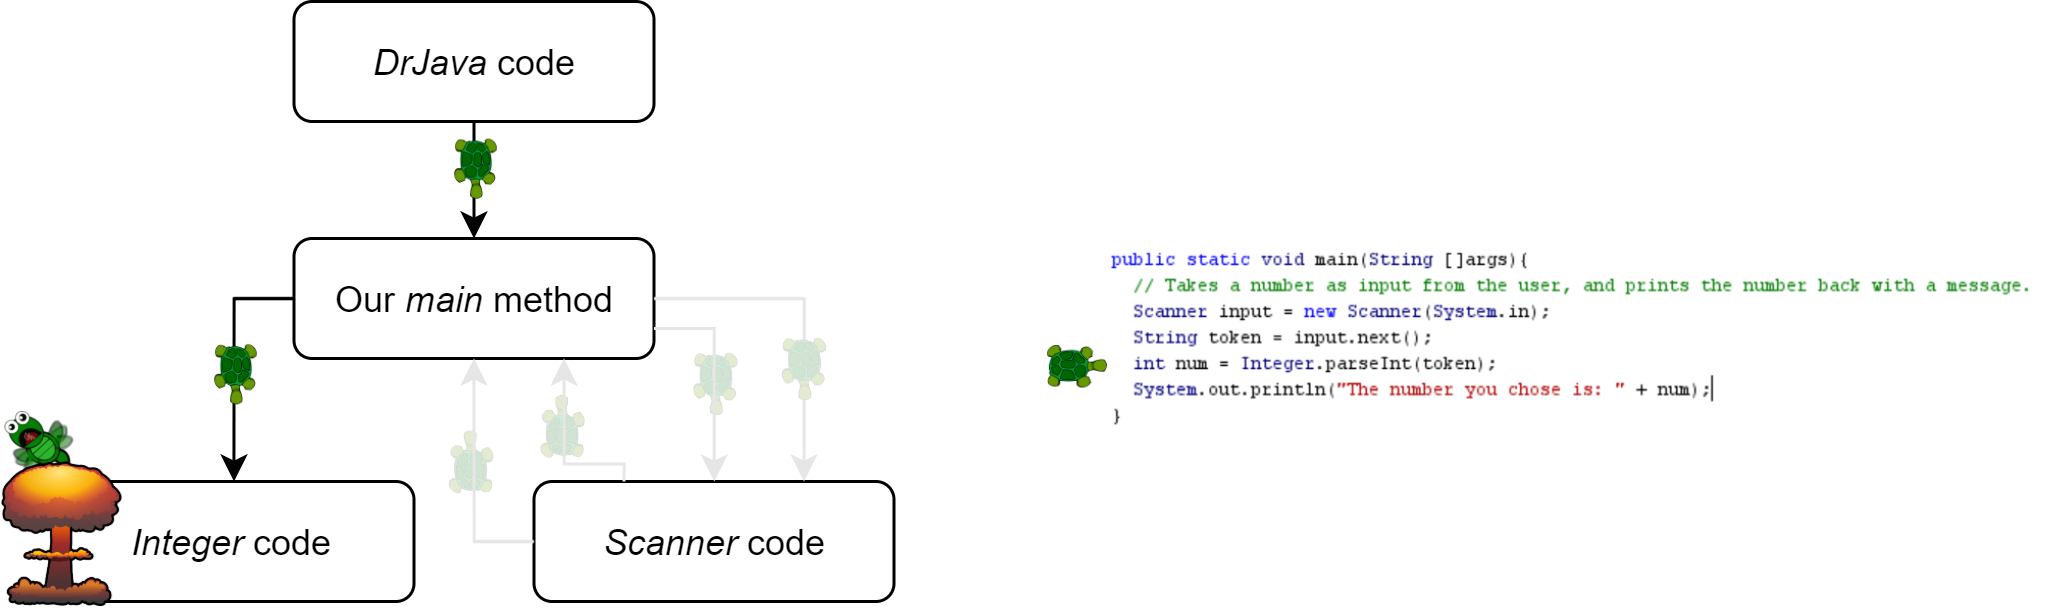
\includegraphics[width=1\textwidth]{images/code_turtle_4.png}
  \caption{}
  \label{fig:sturtle4}
\end{subfigure}%

\caption{The execution of our code. \ref{fig:sturtle1}: Execution enters our \textit{main} method. \ref{fig:sturtle2}: Execution enters the code of \textit{Scanner} to execute "new Scanner(System.in)". After completion, it returns to our \textit{main} method. \ref{fig:sturtle3}: Execution enters \textit{Scanner} code again due to the "input.next()" call, and returns when done. \ref{fig:sturtle4}: Execution enters the code of \textit{Integer} to execute "Integer.parseInt(token)". While there, it encounters an Exception.}
\label{fig:turtles}
\end{figure}



In \ref{fig:sturtle1}, out turtle heads off from whatever code DrJava executes when we click "Run" and enters our code. It starts traversing the code line by line, executing whatever statement is written in each line. In \ref{fig:sturtle2}, the turtle reaches \emph{new Scanner(System.in)} which it needs to execute. This leads the turtle to the code defining \emph{Scanner}, which we're unaware of. The turtle executes whatever lines are written there (there may be many), and then finishes and returns to our code. The turtle continues its journey in \ref{fig:sturtle3} and \ref{fig:sturtle4}, until it reaches the line 

\begin{code}
int num = Integer.parseInt(token);
\end{code}


% In \ref{fig:sturtle3} the turtle goes on to execute the next line. This includes running \emph{input.next()}, and assigning it to the variable token. Since \emph{input} is a \emph{Scanner} variable, the code that's being run when calling \emph{input.next()} is defined in the Scanner code files, and so the turtle makes another trip there and back.

% In \ref{fig:sturtle4} our turtle reaches the offending line, \emph{int num = Integer.parseInt(token)}. To execute it, the turtle heads over to the \emph{Integer} code. Remember that the user gave a wrong input in this execution, and so somewhere in that code our turtle will encounter an exception and stop whatever it was doing.

The stack trace is meant to trace the places our turtle visited on the way to an exception. It ignores any trips the turtle completed successfully, like the two trips to the \emph{Scanner} code. In our case, it should specify the places visited in the DrJava code, our \emph{main} method and the \emph{Integer} code.

The stack trace should be read starting with the bottom line. The bottom five lines all belong to the DrJava code, and in general we can ignore whatever comes below our \emph{main} method, in this case \emph{Snippet.main(Snippet.java:8}. That line tells us that the turtle encountered the exception after visiting line 8 of the \emph{main} method we wrote on the \emph{Snippet} class. The visit to the \emph{Integer} code, and the places the turtle visited there, are traced in the lines above. 

When we write code for bigger projects, our code can become very long, and be separated to many functions and written over many files. An execution can also pass through the same line of code more than once, arriving from different places each time. The stack trace can help us pinpoint the place our code failed at, and figure out how it got there.

% Notice that sometimes the compiler can catch problems that only might happen during compilation. In these cases, it will notify use during compile time.
% public class Snippet{
%     public static void main(String []args){
%       Scanner input = new Scanner(System.in);
%       String userNumber = input.next();
%       int weight = Integer.parseInt(userNumber);
      
%       String response;
%       if(weight > 25){
%         response = "good";
%       }
%       System.out.println(response);
%     }
% }



% \section{Throwing and Catching Exceptions}

% You can also throw errors, just mention.

\section{Debugging Tactics}

Now that we've goetten familiar with errors, we can talk about different ways by which we can investigate our errors and solve them. If our program has compilation errors, it was never run, and so the error message is all we have to investigate the error with.

Runtime errors and exceptions, however, happen at some point during the program's execution, and they don't necessarily happen every time we run it. Even worse, silent bugs also happen while the program executes, but since those are just the gap between our intentions and the code we wrote, the Java language can't stop and tell us about them when they're encountered.

Before we go on to cover some specific methods for debugging, let's outline the general approach we can take to detect, isolate and fix errors:

\begin{enumerate}
\item Reproduce the error: Find a condition that causes the error to happen. Ideally, understand exactly what conditions causes that.
\item Isolate the error: Find the parts of your code related to the error. If possible, temporarily disable other parts to simplify the program.
\item Identify the cause: Go over your code carefully, and find out how the code behaves differently than you expected it to.
\item Implement and test fix: Re-write your code to take care of the existing problem, then test your code to see that it's working properly.
\end{enumerate}

Different debugging tools and methods relate to the different steps outlined above. For example, unit tests and test driven development (that we'll cover later) help with reproducing, isolating and testing fixes to errors. A debugger is a tool that helps us track the execution of a program (we'll cover jdb, the Java debugger, later), and a profiler helps track the memory consumption and running time of parts in a program.

Here we will focus on the general approach outlined before, and a basic method for debugging called \emph{logging}:

\begin{definition}
\emph{Logging} is the act of printing information about the state of a program while it runs, either to the screen or to a designated \emph{log file}. 
\end{definition}

Logging is an important technique in situations where we can't observe our code as it runs, such as on software that is being run on a system belonging to our client. The information we logged then helps us investigate our program in retrospect. The simplicity of logging, however, allows us to start using it early on in coding, before we learn to use powerful tools like a debugger. Let's try out tackling an error with logging, using this example:

\begin{example}
Look at the following code, that has a bug. Assume the user can be trusted to input only positive integer numbers. 

\begin{code}
import java.util.Scanner;

public class Snippet{
    public static void main(String []args){
        // Get an integer input from the user. Print the product (multiplication) of all positive integers up to this number.
        // If the user gave the numebr n, should return 1 * 2 * ... * n
        int userNum = 0;
        int product = 0;
        String token;
        Scanner input = new Scanner(System.in);
        System.out.println("Please input a number:");
        token = input.next();
        userNum = Integer.parseInt(token);
        
        for(int i = 1; i <= userNum; i++){
            product = product * i;
        }
        
        System.out.println("Product: " + product);
    }
}
\end{code}

\end{example}

We still haven't encountered the error ourselves. As a first step in our investigation, after reading the code, we should reproduce the error. Let's run the code and input different legal values to see what the output is, shown in figure~\ref{fig:bug}.

\begin{figure}[h!]
\centering
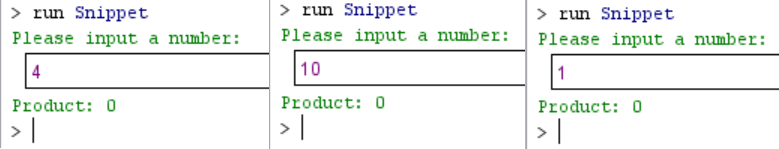
\includegraphics[scale=0.8]{images/bug_outputs.PNG}
\caption{Multiple executions of our program. The correct outputs corresponding to the inputs $4,10$ and $1$ are $24, 3628800$ and $1$.}
\label{fig:bug}
\end{figure}

It seems like the program incorrectly prints $0$ for every input. Now that we've reproduced the error, we want to isolate it. Our program prints the value of the variable \ic{product}. That variable is supposed to hold the product of the numbers between $1$ and \ic{userNum}. Let's focus on the loop that updates \ic{product}:

\begin{code}
for(int i = 1; i <= userNum; i++){
    product = product * i;
}
\end{code}

It seems to multiply the variable by all numbers up to \ic{userNum}, as needed. We can use logging to track the value of this variable throughout the program's run, like this:

\begin{code}
import java.util.Scanner;

public class Snippet{
    public static void main(String []args){
        // Get an integer input from the user. Print the product (multiplication) of all positive integers up to this number.
        // If the user gave the numebr n, should return 1 * 2 * ... * n
        int userNum = 0;
        int product = 0;
        System.out.println("Value of product after initialization: " + product);
        String token;
        Scanner input = new Scanner(System.in);
        System.out.println("Please input a number:");
        token = input.next();
        userNum = Integer.parseInt(token);
        System.out.println("Value of product after taking user input: " + product);
        
        for(int i = 1; i <= userNum; i++){
            product = product * i;
            System.out.println("Value of product after loop iteration: " + product);
        }
        
        System.out.println("Product: " + product);
    }
}
\end{code}

Running this program with the input $3$ results in the output shown in figure~\ref{fig:logging}. 

\begin{figure}[h!]
\centering
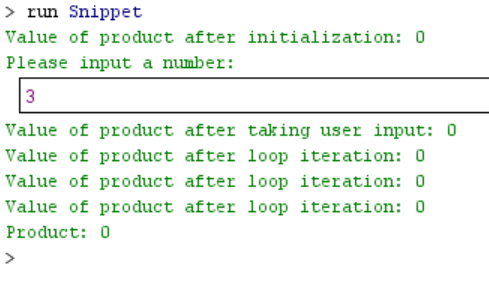
\includegraphics[scale=0.8]{images/logging.PNG}
\caption{Running the program with logging.}
\label{fig:logging}
\end{figure}

We can see that the value of \ic{product} was $0$ throughout the execution of the program. This explains why the value didn't change between iterations of the loop -- multiplying $0$ by any number results in $0$. We thus know that the problem must originate from the initialization of \ic{product}: 

\begin{code}
int product = 0;
\end{code}

Now we know the cause of the problem. Initializing \ic{product} to $0$ made all the multiplications later useless, since the value remained $0$. 

We can now implement a fix to the problem, by initializing \ic{product} with a value that will allow it to change between iterations of the loop. Since we are already supposed to multiply with all the numbers up to \ic{userNum}, we can choose $1$ for the initial value, which is neutral to the multiplication.  After implementing the change, all that's left is to check the new outputs of the program, by running it again with different inputs.

Later in the course, our toolbox for debugging will grow. Logging by printing values, however, can serve us in the meantime to implement the general approach for finding and fixing errors, as we outlined above.


we should figure out \emph{when} that variable 


It's important, then, that we have a way of investigating our code as it runs. One of the common and powerful methods of doing that is called \emph{step debugging}, 

Even worse, silent bugs happen 

and runtime errors and exceptions, we can start by reading the error messages and stack traces. 

% Talk about preventive programming? (tests, coding patterns and design principles)

% Mention rubberducking?

\section{Closing words}

Debugging is an unrewarding process. when you write code, you see the fruits of your labour -- hours of work transform to lines of code, your will made real for the computer. When you debug, you spend your time, sometimes days, just to end up with a code that does what it was supposed to do when you started.

This is not wasted time, however. This is an important counterpart to writing code, and one that every programmer has to go through.

\begin{mdframed}
% "To err is human, to fix your bugs divine. " -- Stackoverflow user Ward Muylaert

% "Human beings are incapable of avoiding errors. You might as well be embarrassed that you have a nose." from https://www.cis.upenn.edu/~matuszek/General/JavaSyntax/errors.html?


“If debugging is the process of removing software bugs, then programming must be the process of putting them in.” ― Edsger W. Dijkstra

\end{mdframed}

Programmers typically spend half of their programming time debugging\footnote{Britton, Tom, et al. "Reversible debugging software." Judge Bus. School, Univ. Cambridge, Cambridge, UK, Tech. Rep (2013).}. With more practice and better debugging habits, you could make that process more efficient. Regardless, reward yourself when you fix a bug -- it might be invisible, but you're making progress.